\documentclass{article}
\usepackage{polski}
\usepackage[utf8]{inputenc}
\usepackage{cite}
\usepackage{indentfirst}
\usepackage{url}
\usepackage[a4paper]{geometry}
\usepackage{fancyvrb}
\usepackage{hyperref}
\usepackage{listings}
\usepackage{float}
\usepackage{pdfpages}
\lstset{
basicstyle=\small\ttfamily,
columns=flexible,
breaklines=true
}


\usepackage{tikz}
\usetikzlibrary{shapes,arrows,positioning}

\widowpenalty=10000
\clubpenalty=10000

\renewcommand{\labelitemii}{$\circ$}
\begin{document}

\begingroup
    \centering
    \huge\textbf{Using neural networks for popularity prediction of online video content}\\[0.75em]
    \large\textbf{Raport z postępów w pracy inżynierskiej}\\[0.75em]
    \vspace{0.2cm}
    {\large{}\itshape{} Bocheński Tomasz\par{}}
    \vspace{0.5cm}
    {\large \today\par}
\endgroup


\section{Podsumowanie obecnego semestru}
W obecnym semestrze poczyniłem następujące postępy.

\subsection{Wybór źródeł danych do nauki i testowania sieci}
Spośród dostępnych serwisów internetowych z filmikami wybrałem cztery, które moim zdaniem najlepiej nadają się jako źródła danych. Są nimi: Facebook, Youtube, Dailymotion, Vimeo. Wszystkie one cechują się dużą popularnocią, dużą bazą filmików oraz udostępniają API pozwalające na uzyskanie satysfakcjonujących metadanych. Następnie dla każdego z tych serwisów, wspólnie z kolegą, stworzyliśmy listy najbardziej aktywnych użytkowników i kanałów. Poniżej przedstawiam podsumowanie ich ilości:
\begin{itemize}
    \item Youtube: 1120
    \item Facebook: 144
    \item Dailymotion: 865
    \item Vimeo: 49
\end{itemize}
Listy te można znaleźć tutaj:\url{https://github.com/tom3097/VideoPopularityPrediction/tree/master/VideoCrawlers/data}

\subsection{Stworzenie web crawlerów (robotów internetowych)}
Następnie zapoznałem się dokładniej z API przedstawionych powyżej serwisów internetowych oraz napisałem odpowiednie roboty internetowe dla każdego z nich. Poniżej przedstawiam podsumowanie iloci filmików dla których metadane zostały pobrane wraz z ich całkowitą wielkocią (bez uwzględnienia filtrowania):
\begin{itemize}
    \item Youtube: liczba filmików - 419046, calkowity rozmiar - 1.8 GB
    \item Facebook: liczba filmików - 195945, calkowity rozmiar - 922 MB
    \item Dailymotion: liczba filmików - 1811543, calkowity rozmiar - 3GB
    \item Vimeo: liczba filmików - 98078, calkowity rozmiar - 897 MB
\end{itemize}
Oraz przykładowe metadane uzyskane dla jednego pliku video dla każdego z serwisów internetowych:

\begin{itemize}
    \item Youtube:
\end{itemize}
\begin{Verbatim}
{
        "channel_UC": "UCzzYnZ8GIzfB1Vr3hk2Nj9Q", 
        "date_time": "2016-05-21 09:17:32", 
        "etag": "\"zekp1FB4kTkkM-rWc1qIAAt-BWc/PlH3kUy4HPS_G2mFNvMXGuQMgmQ\"", 
        "id": "cNeU6QbejDs", 
        "kind": "youtube#video", 
        "snippet": {
            "categoryId": "22", 
            "channelId": "UCzzYnZ8GIzfB1Vr3hk2Nj9Q", 
            "channelTitle": "Tiger Fitness", 
            "description": "SUPPORT MARC LOBLINER'S COMPANY AND SHOP 
            AT TIGERFITNESS.COM! http://www.tigerfitness.com\n\nMarc and 
            The Hollywood Militia NOW OFFER COACHING Email mlobliner@gmail.com 
           or john.hollywood.tcoach@gmail.com\n\nTHE INTRO AND OUTRO SONG!"
            "liveBroadcastContent": "none", 
            "localized": {
                "description": "SUPPORT MARC LOBLINER'S COMPANY AND SHOP AT
                TIGERFITNESS.COM!",
                "title": "Creatine While Cutting"
            }, 
            "publishedAt": "2013-07-23T20:40:57.000Z", 
            "tags": [
                "muscle and fitness", 
                "work out routines", 
                "tigerfitness.com", 
                "ethitech nutrition", 
                "marc lobliner", 
                "Lobliner", 
                "machine", 
                "mts nutrition"
            ], 
            "thumbnails": {
                "default": {
                    "height": 90, 
                    "url": "https://i.ytimg.com/vi/cNeU6QbejDs/default.jpg", 
                    "width": 120
                }, 
                "high": {
                    "height": 360, 
                    "url": "https://i.ytimg.com/vi/cNeU6QbejDs/hqdefault.jpg", 
                    "width": 480
                }, 
                "maxres": {
                    "height": 720, 
                    "url": "https://i.ytimg.com/vi/cNeU6QbejDs/maxresdefault.jpg", 
                    "width": 1280
                }, 
                "medium": {
                    "height": 180, 
                    "url": "https://i.ytimg.com/vi/cNeU6QbejDs/mqdefault.jpg", 
                    "width": 320
                }, 
                "standard": {
                    "height": 480, 
                    "url": "https://i.ytimg.com/vi/cNeU6QbejDs/sddefault.jpg", 
                    "width": 640
                }
            }, 
            "title": "Creatine While Cutting"
        }, 
        "statistics": {
            "commentCount": "192", 
            "dislikeCount": "20", 
            "favoriteCount": "0", 
            "likeCount": "1247", 
            "viewCount": "79760"
        }
}
\end{Verbatim}

\begin{itemize}
    \item Facebook:
\end{itemize}
\begin{Verbatim}
{
        "content_category": "NEWS",
        "created_time": {
            "date": "2016-02-25 12:00:00.000000",
            "timezone_type": 1,
            "timezone": "+00:00"
        },
        "description": "What do you want to know about the Syrian war and the refugee 
         crisis? On The Line will take your questions today at 12pm ET.\n\nWe want to
         hear from you. Let us know your thoughts on Twitter with #ontheline, or send 
         us a video message on Skype. http://bit.ly/1KLAjOD",
        "from": {
            "name": "VICE News",
            "id": "235852889908002"
        },
        "id": "557585337734754",
        "length": 32.064,
        "permalink_url": "/vicenews/videos/557585337734754/",
        "picture": "https://scontent.xx.fbcdn.net/hvthumb-xpt1/v/t15.0-10/p128x128/
        12323142_557586267734661_590161308_n.jpg?oh=4ccb2de17f95ed1be7d4e0ac
        64975ceb&oe=57795653",
        "source": "https://video.xx.fbcdn.net/hvideo-xpt1/v/t43.1792-2/12741453_4337
        98730149138_852895459_n.mp4?efg=eyJybHIiOjE1MDAsInJsYSI6MTAyNCwidmV
        uY29kZV90YWciOiJzdmVfaGQifQ%3 %3D&rl=1500&vabr=505&oh=bf736e8
        3d68e1c9f7d7fe342e004da47&oe=56FC2AA0",
        "updated_time": {
            "date": "2016-02-25 12:00:03.000000",
            "timezone_type": 1,
            "timezone": "+00:00"
        },
        "thumbnails": [
            {
                "id": "557586204401334",
                "height": 720,
                "scale": 1,
                "uri": "https://scontent.xx.fbcdn.net/hvthumb-xft1/v/t15.0-10/12672212_5
                57586237734664_1816489778_n.jpg?oh=c5e8ec4a17cce1f081fc90c8dcf
                de335&oe=577E8458",
                "width": 1280,
                "is_preferred": false
            },
            {
                "id": "557586264401328",
                "height": 720,
                "scale": 1,
                "uri": "https://scontent.xx.fbcdn.net/hvthumb-xpt1/v/t15.0-10/12323142_
                557586267734661_590161308_n.jpg?oh=2ee8e40bccbc066c76376a69fe8a
                52d3&oe=5789F700",
                "width": 1280,
                "is_preferred": true
            }
        ],
        "likesCount": 21,
        "commentsCount": 8,
        "sharedpostsCount": null,
        "viewCount": 2470,
        "time_date": "28-03-16 21:35:23",
        "page_name_id": "vicenews"
}
\end{Verbatim}

\begin{itemize}
    \item Dailymotion:
\end{itemize}
\begin{Verbatim}
{
        "allow_comments": true, 
        "aspect_ratio": 1.7777777910233, 
        "available_formats": [
            "l1", 
            "l2", 
            "ld", 
            "sd", 
            "hq", 
            "hd720", 
            "hd1080"
        ], 
        "bookmarks_total": 0, 
        "comments_total": 0, 
        "country": "CN", 
        "created_time": "2016-03-24 15:21:33", 
        "date_time": "2016-03-24 22:06:18", 
        "description": "Jakis opis", 
        "duration": 892, 
        "embed_url": "http://www.dailymotion.com/embed/video/x3zv9ds", 
        "filmstrip_60_url": "http://static2.dmcdn.net/static/video/485/346/2
        41643584:jpeg_preview_contact.jpg?20160324230220", 
        "id": "x3zv9ds", 
        "language": "zh", 
        "name_id": "zjtv", 
        "owner.id": "x1jfqu5", 
        "sprite_320x_url": "http://s2.dmcdn.net/U20VK/320x-rAB.jpg", 
        "tags": [
            "\u4e2d\u56fd\u68a6\u60f3\u79c0", 
            "\u5468\u7acb\u6ce2", 
            "\u6d59\u6c5f\u536b\u89c6", 
            "\u4e2d\u56fd\u68a6\u60f3\u79c0 0324", 
            "\u4e2d\u56fd\u68a6\u60f3\u79c02016", 
            "zhoulibo"
        ], 
        "thumbnail_url": "http://s2.dmcdn.net/U2zrm.jpg", 
        "title": "\u4e2d\u56fd\u68a6\u60f3\u79c0 \u7b2c9\u5b63 20160324\u671f:\u6b66
        \u672f\u8857\u821e\u521b\u610f\u878d\u5408\u5f70\u663e\u522b\u6837
        \u4e2d\u56fd\u98ce", 
        "url": "http://www.dailymotion.com/video/x3zv9ds_%E4%B8%AD%E5%9B
        %BD%E6%A2%A6%E6%83%B3%E7%A7%80-%E7%AC%AC9%E5%AD
        %A3-20160324%E6%9C%9F-%E6%AD%A6%E6%9C%AF%E8%A1%97
        %E8%88%9E%E5%88%9B%E6%84%8F%E8%9E%8D%E5%90%88%
        E5%BD%B0%E6%98%BE%E5%88%AB%E6%A0%B7%E4%
        B8%AD%E5%9B%BD%E9%A3%8E_tv", 
        "views_last_day": 8, 
        "views_last_hour": 0, 
        "views_last_month": 8, 
        "views_last_week": 8, 
        "views_total": 8
}
\end{Verbatim}

\begin{itemize}
    \item Vimeo:
\end{itemize}
\begin{Verbatim}
{
        "created_time": "2009-11-12T01:28:03+00:00", 
        "date_time": "2016-03-25 19:58:14", 
        "description": "cast ELIZA TAYLOR and TIM ROSS\nwriter director TIMOTHY
         MELVILLE\nproducer DOMINIC ALLEN\ncinematographer JOEL BETTS\nproduction
         company SCARAB STUDIO FILMS. 2009\n\nDownload the script here, http://tinyurl.
         com/kezzws4\nView the Spanish dub here, http://youtu.be/eYTJdv0JMhw\n\nOfficial
         Selection Flickerfest 2010\nOfficial Selection St Kilda Film Festival 2010\nOfficial 
        Selection Dungog Film Festival 2010\nWinner Best Film Hillside Film
        "duration": 397, 
        "height": 640, 
        "language": null, 
        "link": "https://vimeo.com/timothymelville/thelaundromat", 
        "metadata": {
            "connections": {
                "comments": {
                    "options": [
                        "GET", 
                        "POST"
                    ], 
                    "total": 122, 
                    "uri": "/videos/7563705/comments"
                }, 
                "credits": {
                    "options": [
                        "GET", 
                        "POST"
                    ], 
                    "total": 3, 
                    "uri": "/videos/7563705/credits"
                }, 
                "likes": {
                    "options": [
                        "GET"
                    ], 
                    "total": 2311, 
                    "uri": "/videos/7563705/likes"
                }, 
                "pictures": {
                    "options": [
                        "GET", 
                        "POST"
                    ], 
                    "total": 1, 
                    "uri": "/videos/7563705/pictures"
                }, 
                "related": {
                    "options": [
                        "GET"
                    ], 
                    "uri": "/channels/iphones/videos?fields=stats,description,language,privacy
                    ,pictures,duration,tags,uri,modified_time,height,width,link,created_time,
                    name,user.uri,metadata&per_page=50&page=1&sort=date&direction=
                    asc&offset=1"
                }, 
                "texttracks": {
                    "options": [
                        "GET", 
                        "POST"
                    ], 
                    "total": 2, 
                    "uri": "/videos/7563705/texttracks"
                }
            }, 
            "interactions": {
                "like": {
                    "added": false, 
                    "added_time": null, 
                    "uri": "/users/49719331/likes/7563705"
                }, 
                "watchlater": {
                    "added": false, 
                    "added_time": null, 
                    "uri": "/users/49719331/watchlater/7563705"
                }
            }
        }, 
        "modified_time": "2016-03-25T19:11:25+00:00", 
        "name": "The Laundromat | Short Film", 
        "name_id": "iphones", 
        "pictures": {
            "active": true, 
            "sizes": [
                {
                    "height": 480, 
                    "link": "https://i.vimeocdn.com/video/133977185_960x480.jpg?r=pad", 
                    "width": 960
                }, 
                {
                    "height": 640, 
                    "link": "https://i.vimeocdn.com/video/133977185_1280x640.jpg?r=pad", 
                    "width": 1280
                }
            ], 
            "type": "custom", 
            "uri": "/videos/7563705/pictures/133977185"
        }, 
        "privacy": {
            "add": true, 
            "comments": "anybody", 
            "download": false, 
            "embed": "public", 
            "view": "anybody"
        }, 
        "stats": {
            "plays": 167662
        }, 
        "tags": [
            {
                "canonical": "shortfilm", 
                "metadata": {
                    "connections": {
                        "videos": {
                            "options": [
                                "GET"
                            ], 
                            "total": 188589, 
                            "uri": "/tags/shortfilm/videos"
                        }
                    }
                }, 
                "name": "Short Film", 
                "tag": "Short Film", 
                "uri": "/tags/shortfilm"
            }
        ], 
        "uri": "/videos/7563705", 
        "user": {
            "uri": "/users/2621541"
        }, 
        "width": 1280
}
\end{Verbatim}


Roboty internetowe (wraz  ich opisem) można znaleźć tutaj: \url{https://github.com/tom3097/VideoPopularityPrediction/tree/master/VideoCrawlers/src}. Dużym problemem było znalezienie bezporednich url'i do filmików dla Youtube, Dailymotion oraz Vimeo. Ostatecznie udało mi się to osiągąć za pomocą narzędzie youtube-dl, które można znaleźć tutaj:  \url{https://github.com/rg3/youtube-dl}. Jednak wykorzystanie tego narzędia drastycznie zwiększa czas działania crawlerów, ponadto linki są aktywne tylko przez pewien czas. Z tego powodu zdecydowałem się nie korzystać z niego do czasu, gdy url'e te będą mi rzeczywicie potrzebne.

\subsection{Zapoznanie się z architekturą sztucznych sieci neuronowych}
Ponieważ dotychczas nie miałem nic wspólnego z sieciami neuronowymi, musiałem poświęcić trochę czasu aby zapoznać się z ich podstawowymi zagadnieniami oraz ich architekturą. W pierwszym kroku zapoznałem się z podstawami "regularnych" sieci neuronowych. Następnie poznałem architekturę ConvNet. Wiedzę zdobywałem z tutoriala który można znaleźć tutaj: \url{http://cs231n.github.io/}. Ponadto zacząłem internetowe kursy \url{https://www.udacity.com/course/deep-learning--ud730} oraz \url{https://www.coursera.org/learn/machine-learning} (których jeszcze nie skończylem, jednak pomogły mi zrozumieć podstway).


\subsection{Zapoznanie się z frameworkiem Caffe}
Aby zapoznać się z Caffe przeczytałem oficjalną dokumentację, którą można znaleźć na ich stronie, bazując głównie na \url{http://caffe.berkeleyvision.org/tutorial/} oraz w mniejszym stopniu również na innych dokumentach.

\subsection{Zapoznanie się z niezbędnymi API w Pythonie (Caffe, LMDB, numpy)}
W tym celu przeanalizowałem niektóre z plików typu IPython Notebook które można znaleźć tutaj:  \url{https://github.com/BVLC/caffe/tree/master/examples}. Wynikiem tych analiz były pewne skrypty implementujące sieci neuronowe, skrypty to ich testowania, używania itp. Nie stanowiły one jednak wartości "materialnej", służyły tylko mojemu zapoznaniu się, dlatego nie udostępniłem ich na repozytorium.

\subsection{Normalizacja popularności filmików}
Biorąc pod uwagę metadane, które dostępne są na każdym z czterech serwisów internetowych, czyli:
\begin{itemize}
    \item liczba wyświetleń
    \item liczba followersów/subskrypcji dla kanału/użytkownika
    \item data publikacji
\end{itemize}
Wyznaczyłem wzór do normalizacji popularnoci filmików. Wyglada on w następujący sposób
\begin{Verbatim}
normalizedPopularity = log_2( (viewsCount + 1)/followersCount )
\end{Verbatim} 
Poniżej przedstawione zostały przykładowe wykresy popularności dla różnych serwisów: Youtube, Facebook, Dailymotion, Vimeo w miesiącach kolejno: 10.2015, 11.2015, 12.2015, 01.2016.

\begin{figure}[H]
\caption{Youtube: 10.2015, 11.2015, 12.2015, 01.2016}
\centering
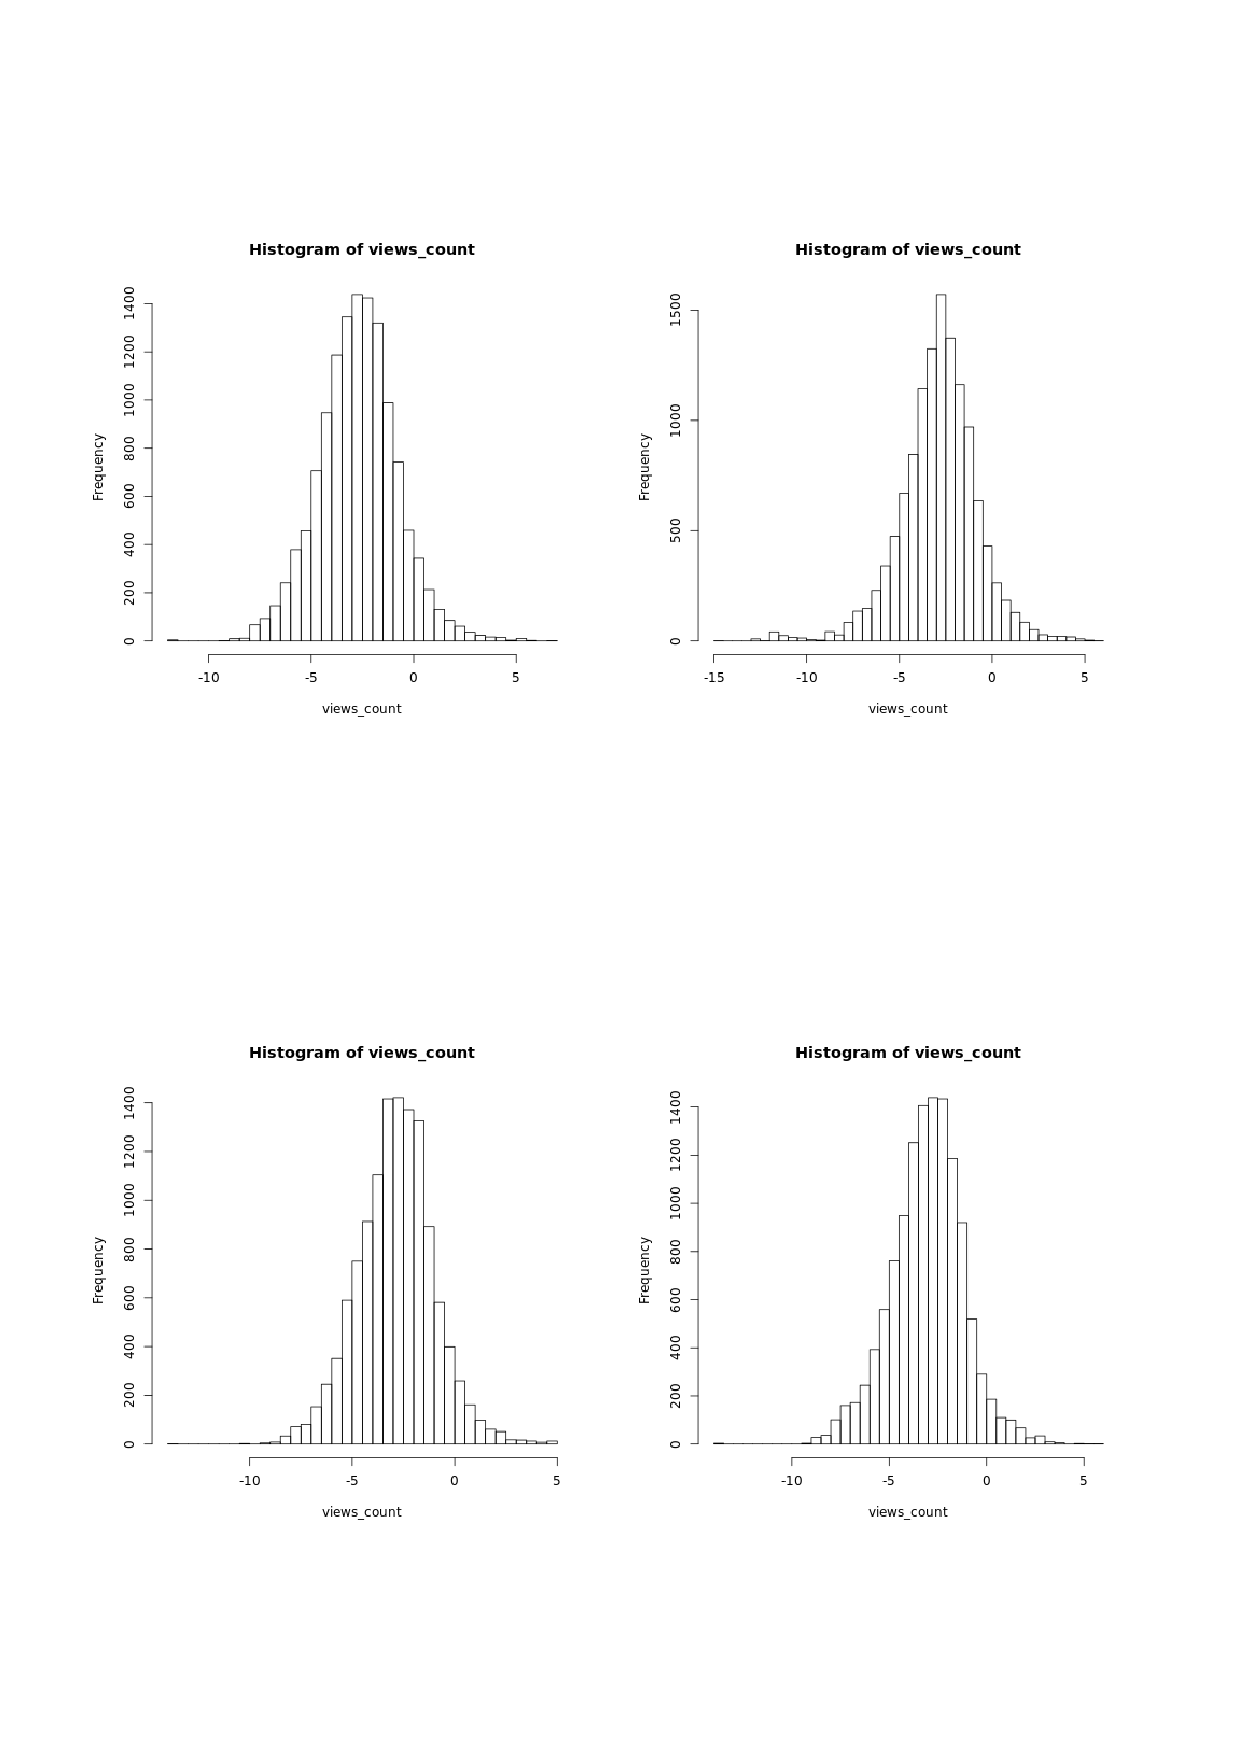
\includegraphics[scale=0.7]{youtubeGauss}
\end{figure}

\begin{figure}[H]
\caption{Facebook: 10.2015, 11.2015, 12.2015, 01.2016}
\centering
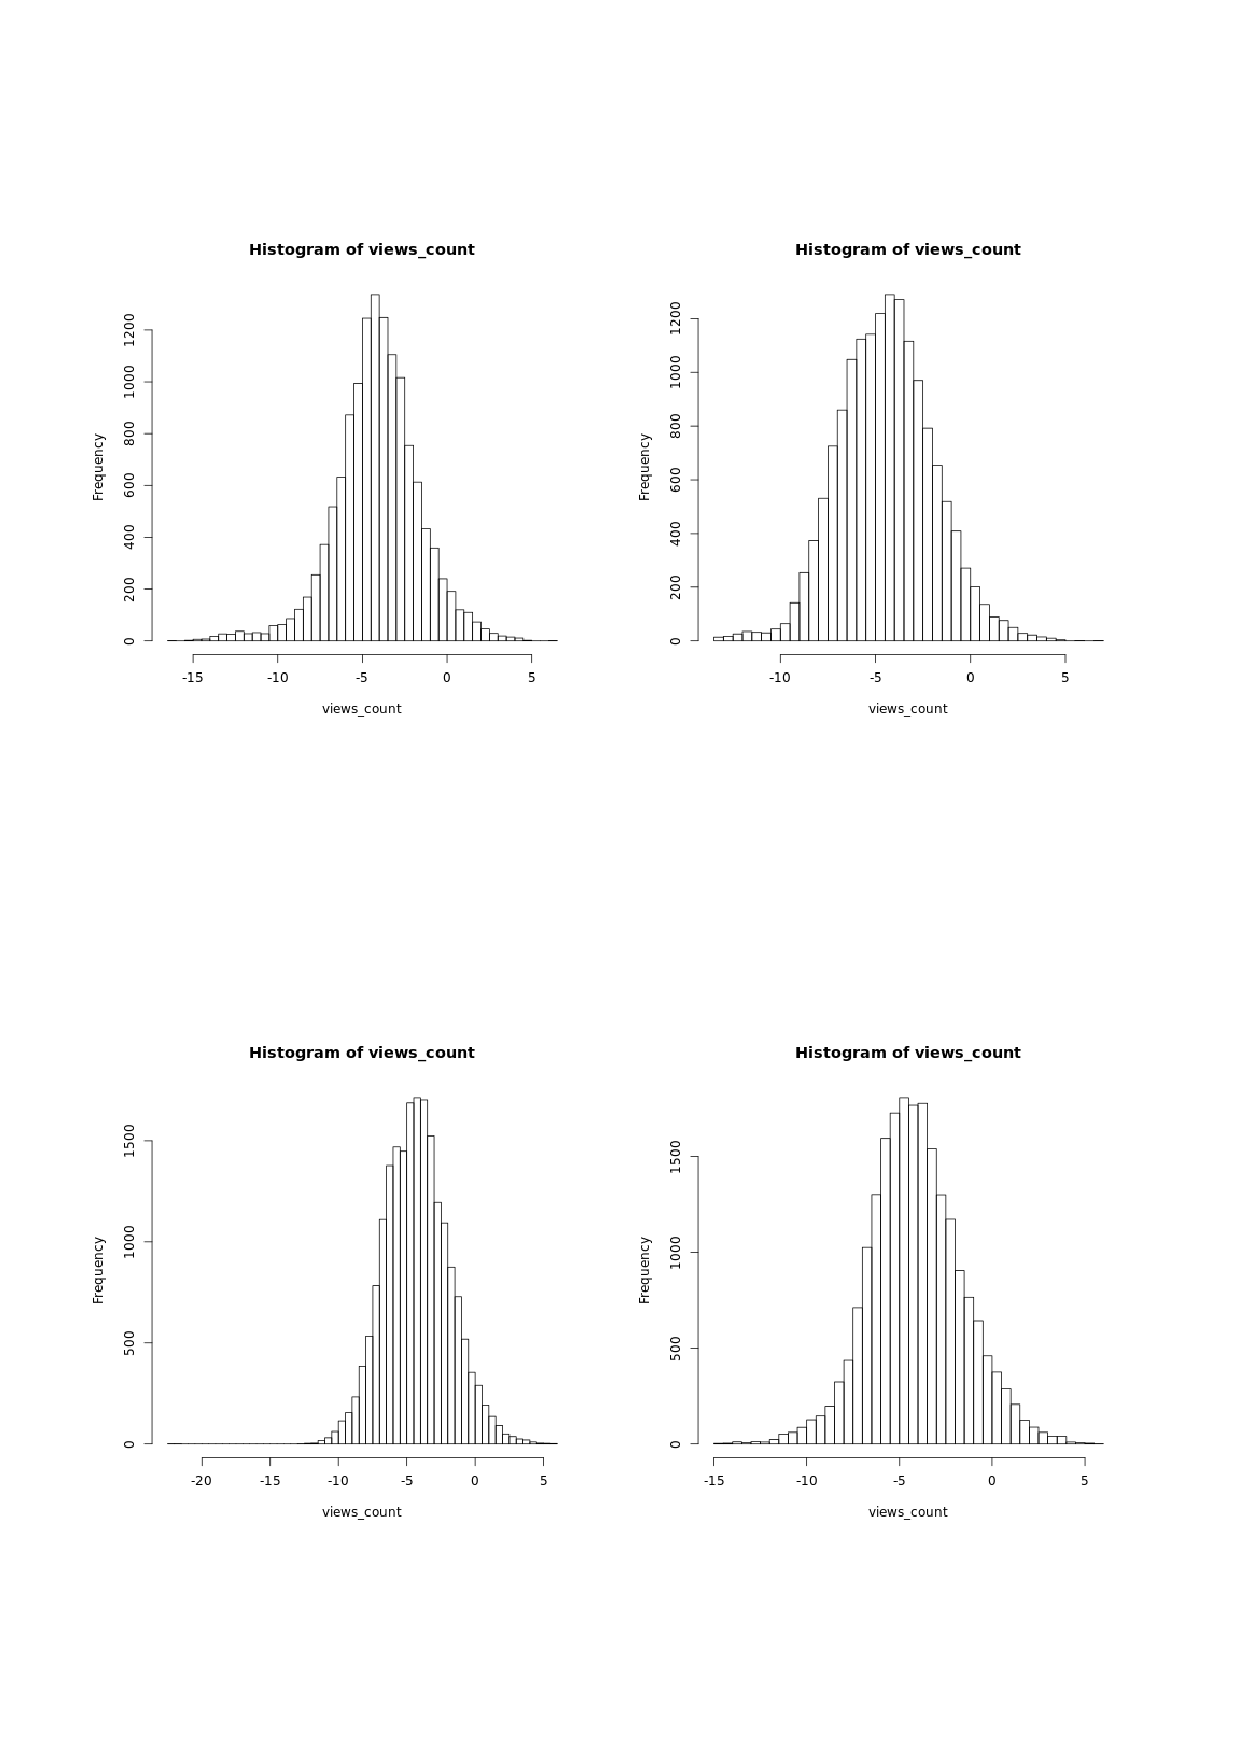
\includegraphics[scale=0.7]{facebookGauss}
\end{figure}

\begin{figure}[H]
\caption{Dailymotion: 10.2015, 11.2015, 12.2015, 01.2016}
\centering
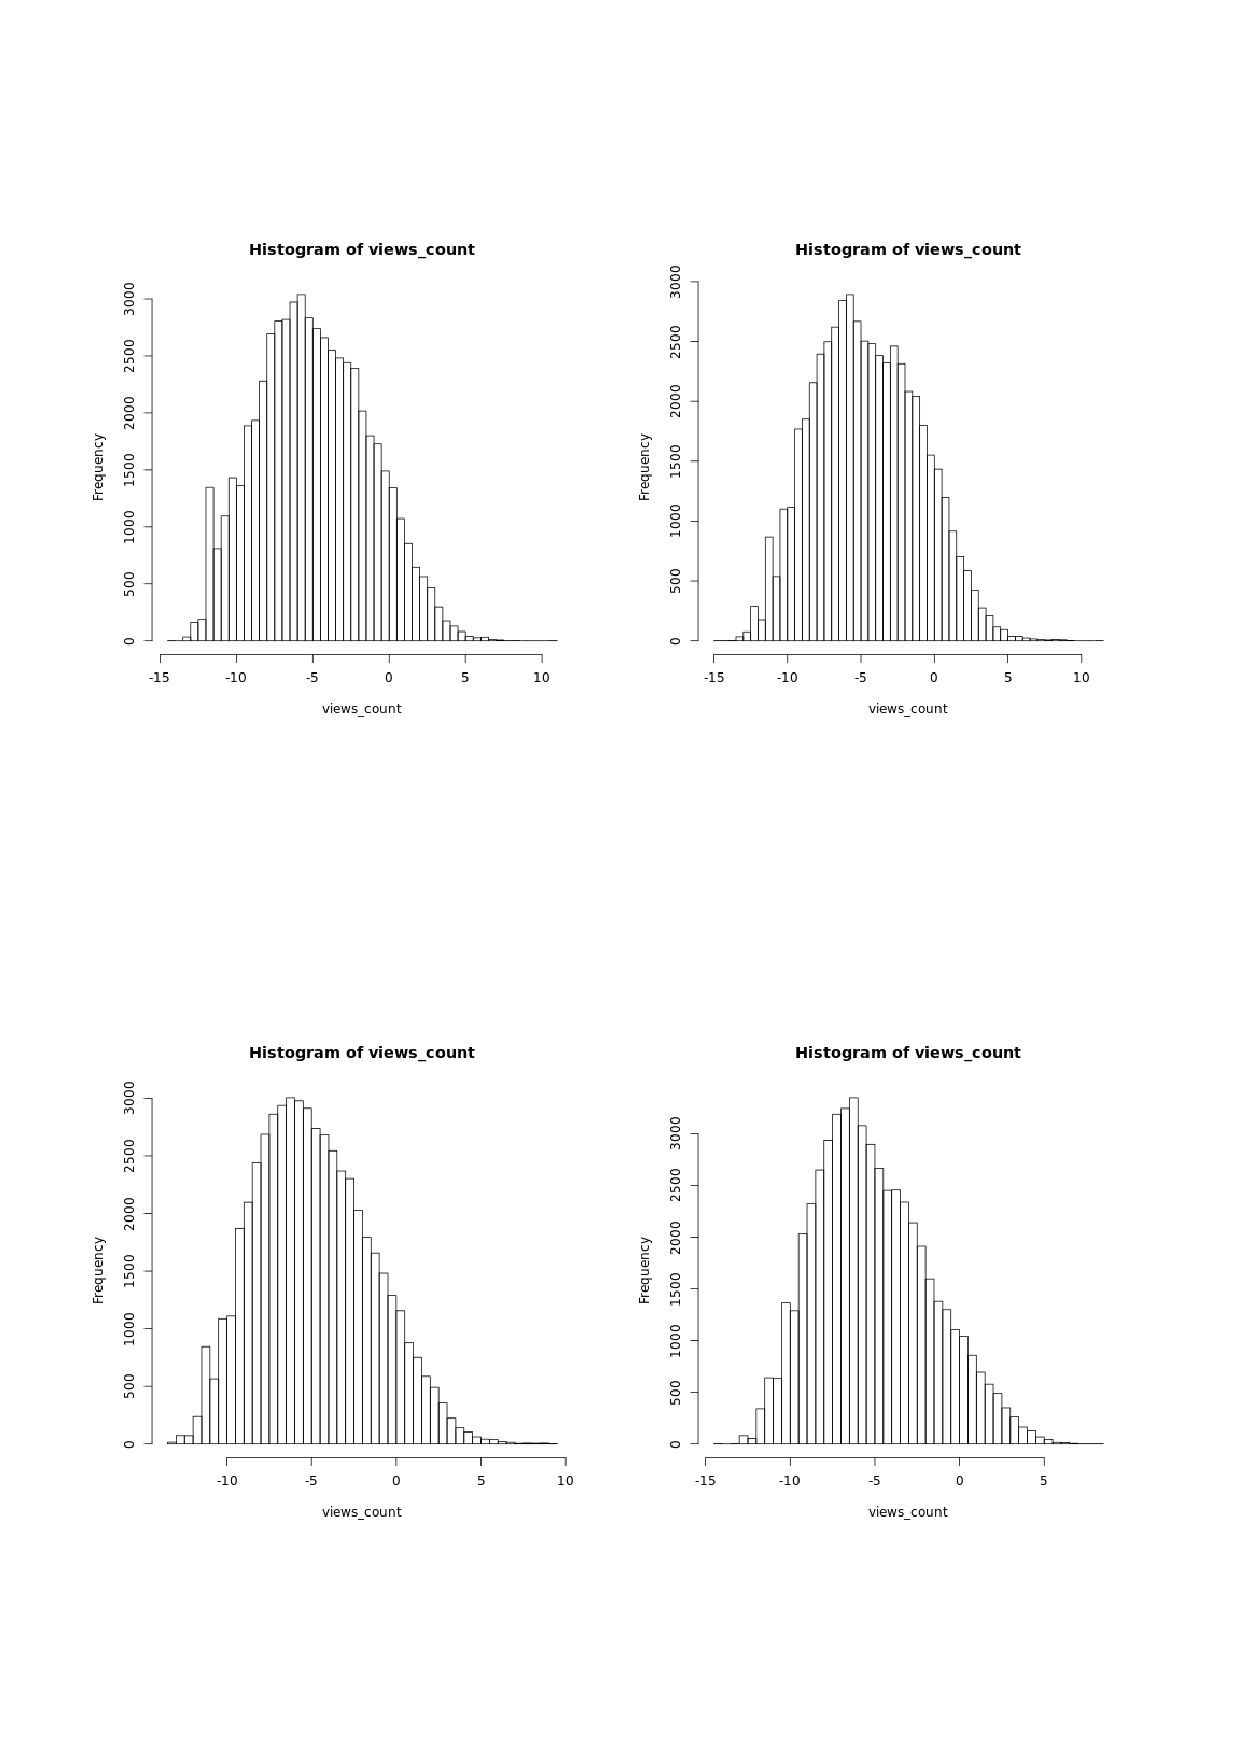
\includegraphics[scale=0.7]{dailymotionGauss}
\end{figure}

\begin{figure}[H]
\caption{Vimeo: 10.2015, 11.2015, 12.2015, 01.2016}
\centering
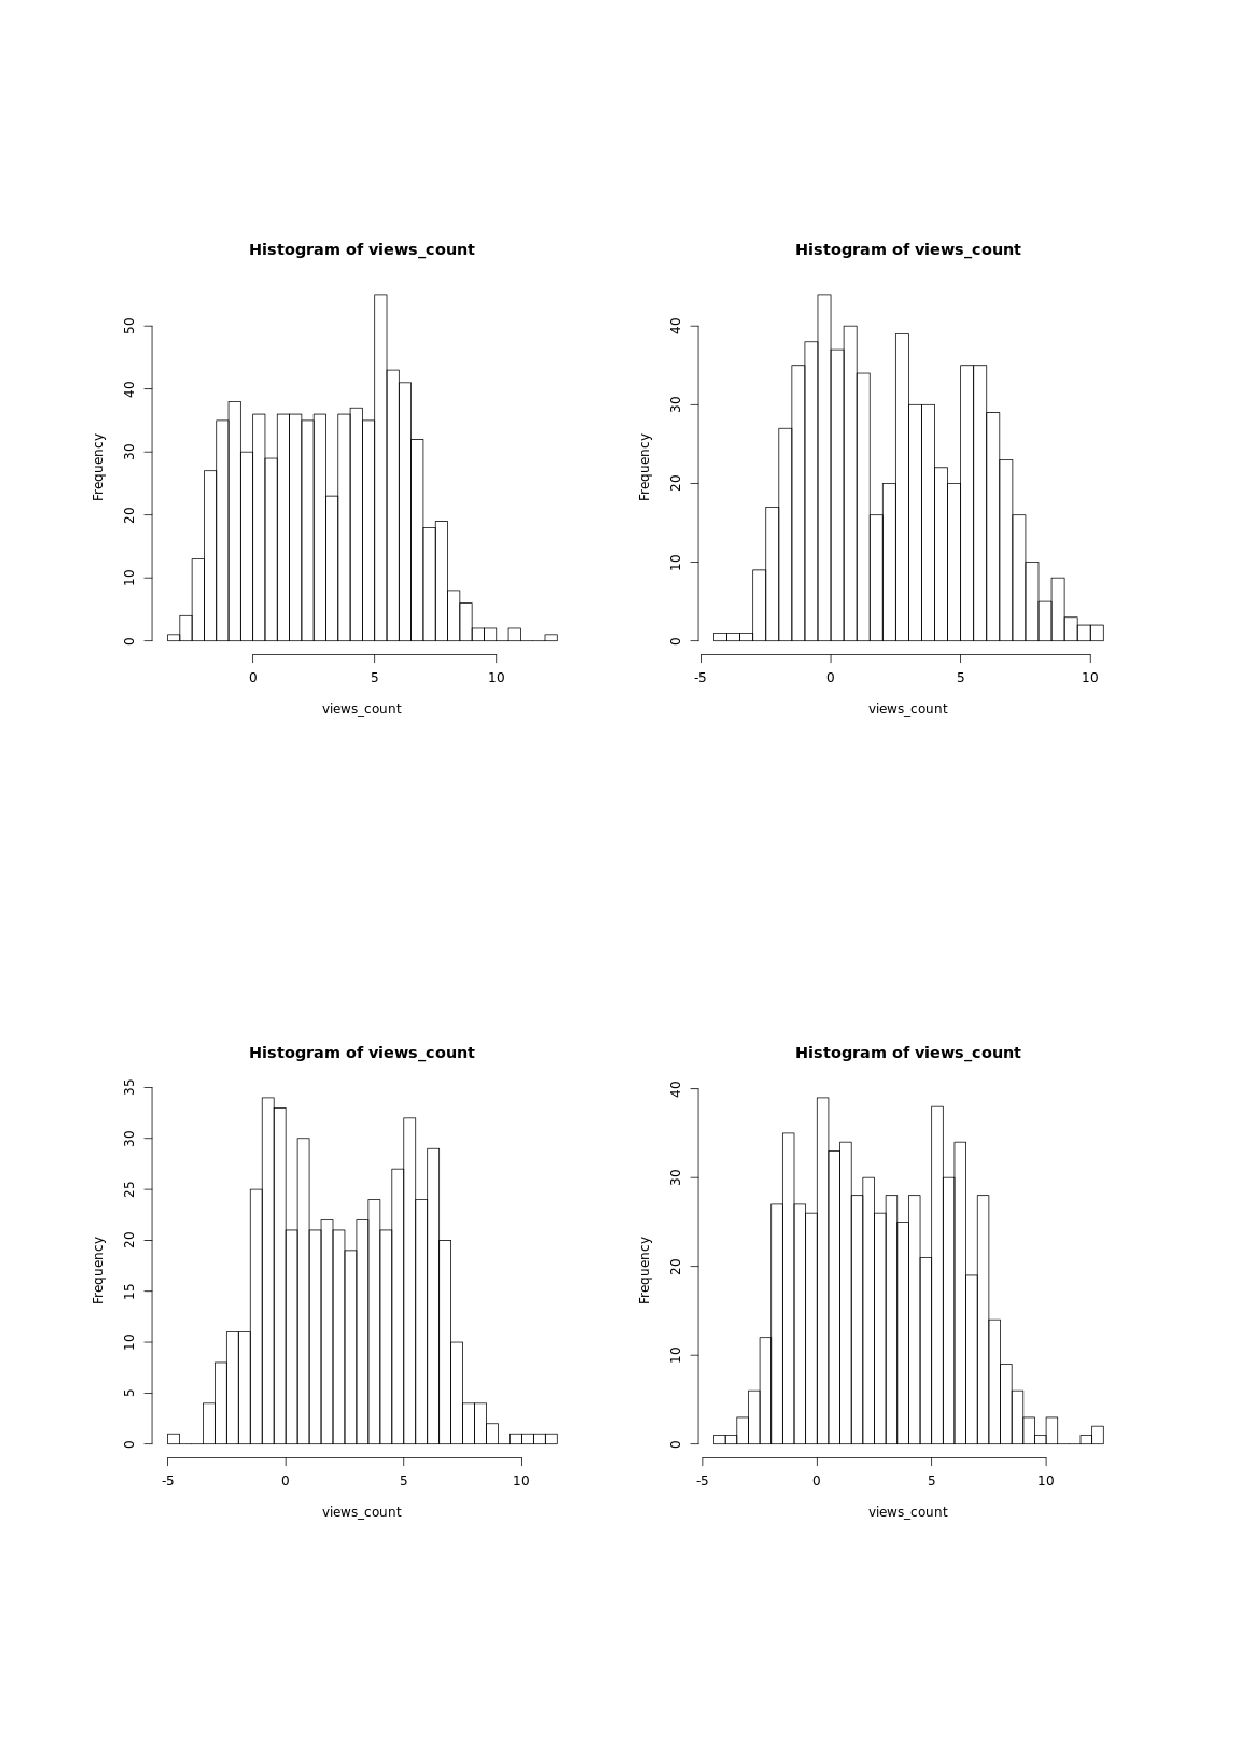
\includegraphics[scale=0.7]{vimeoGauss}
\end{figure}
Jak widać w przypadku filmików z Youtube czy też Facebooka otrzymujemy wykresy gaussowskie, dla filmików z Dailymotion otrzymujemy lekko przesunięte wykresy gaussowskie. Jedynie w przypadku filmików z Vimeo widać większe odstępstwa, jednak są one do zaakceptowania.
Skrypty to tworzenia wykresów, wraz z opisem ich uruchamiania znajdują się tutaj: \url{https://github.com/tom3097/VideoPopularityPrediction/tree/master/GaussTest/src}.

\subsection{Podział filmików na klasy popularności}
Korzystając ze znormalizowanych popularności filmików dokonałem ich podziału na:
\begin{itemize}
    \item dwie klasy popularności (binarnego)
    \item osiem klas popularności
\end{itemize}
Stworzone zostały skrypty do podziału filmików z Youtube oraz Facebooka, jednak podział filmików z Dailymotion oraz Vimeo odbywa się w analogiczny sposób. Skrypty te, wraz z wynikami ich uruchomień, można znaleźć tutaj: \url{https://github.com/tom3097/VideoPopularityPrediction/tree/master/Batches}.

\subsection{Fine-tuning sieci neuronowej}
Aby przeprowadzić fine-tuning, w pierwszej kolejności pobrałem miniaturki filmów z Facebooka (preffered) oraz Youtuba. Skrypty do tego służące znajdują się tutaj: \url{https://github.com/tom3097/VideoPopularityPrediction/tree/master/ThumbDownloaders}. Następnie, korzystając z wytrenowanej wcześniej sieci Berkeley-trained models (\url{https://github.com/BVLC/caffe/tree/master/models/bvlc_reference_caffenet}) przeprowadziłem fine-tuning zarówno dla binarnej klasyfikacji filmików jak i dla podziału na 8 kategorii. W przypadku Facebooka dla klasyfikacji binarnej otrzymałem:
\begin{itemize}
    \item accurancy = 0.60312
    \item loss = 0.651064
\end{itemize}
Natomiast w przypadku podziału na 8 kategorii rezultaty prezentują się następująco:
\begin{itemize}
    \item accurancy = 0.2064
    \item loss = 1.97498
\end{itemize}
Użyte pliki takie jak solvery, definicje sieci można znaleźć tutaj: \url{https://github.com/tom3097/VideoPopularityPrediction/tree/master/Nets}.

\subsection{Wybór najlepszych i najgorszych miniaturek}
W celu wybrania najlepszych i najgorszych miniaturek podłączyłem ostatnią warstwę typu FC na output. Korzystałem z wytrenowanej w poprzednim punkcie sieci za pomocą fine-tuningu dla podziału na 8 kategorii. Ponieważ kategoria 7 grupuje filmiki najbardziej popularne, posortowałem wyniki malejąco wegług punktów przyznanych tej kategorii. W ten sposób otrzymałem najlepsze miniaturki filmików. Analogicznie postąpiłem w przypadku wyznaczenia najgorszych miniaturek. Poniewaz kategoria 0 grupuje filmiki najmniej popularne, również posortowałem wyniki malejąco według tej kategorii, w tym przypadku otrzymując jednak najgorsze miniaturki filmików. Poniżej przedstawiam przykładowe 4 najlepsze i 4 najgorsze miniaturki wyznaczoych ze zboru danych do testowania.

\begin{figure}[H]
\caption{Przykładowe 4 najlepsze miniaturki}
\centering
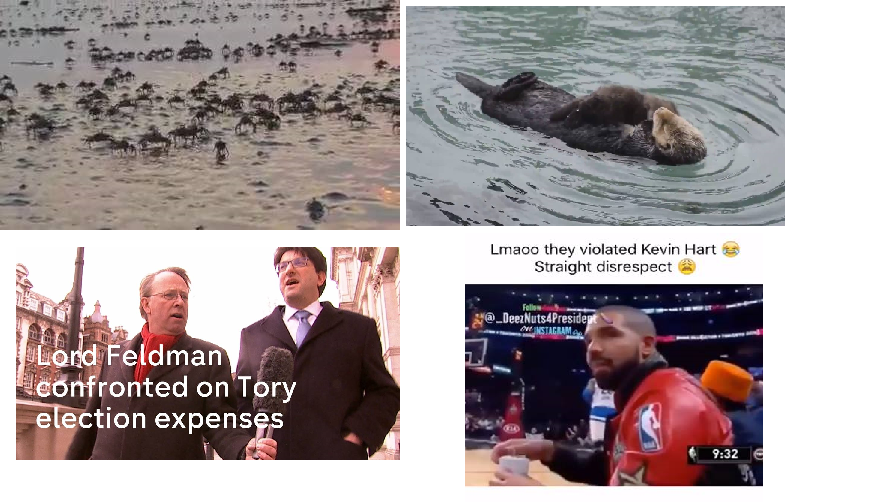
\includegraphics[scale=0.7]{bestThumbs}
\end{figure}

\begin{figure}[H]
\caption{Przykładowe 4 najgorsze miniaturki}
\centering
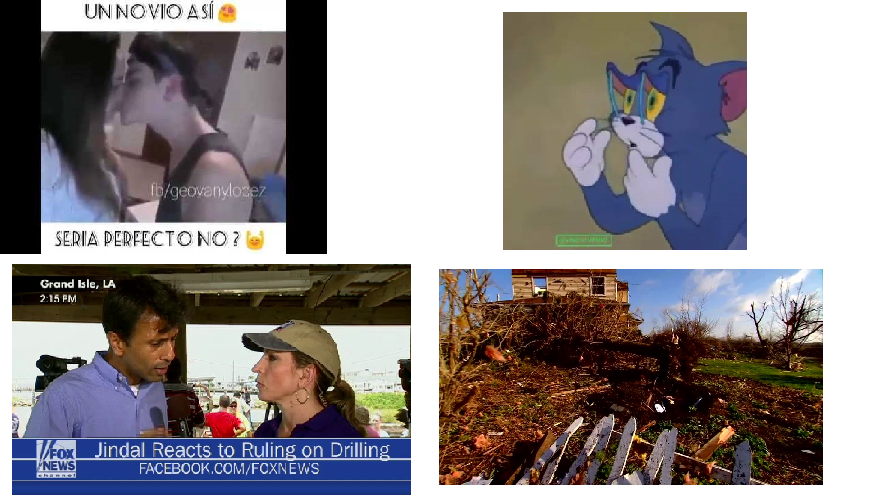
\includegraphics[scale=0.7]{worstThumbs}
\end{figure}

Skrypt użyty do wyznaczenia tych miniaturek można znaleźć tutaj: \url{https://github.com/tom3097/VideoPopularityPrediction/tree/master/BestWorstThumb}. Jak widać, chociaż miniaturka jest ważnym czynnikiem decydującym o popularności pliku video, nie jest ona czynnikiem decydującym.

\subsection{Inne}
Dodatkowo, specjalnie na potrzeby pracy inżynierskiej, nauczyłem się języka R (z którego potem korzystałem na równi z Pythonem). Zapoznałem się również z artykułami które otrzymałem, można je znaleźć tutaj: \url{https://github.com/tom3097/VideoPopularityPrediction/tree/master/Materials/research_papers}.

\section{Plany na następny semestr}
W następnym semestrze planuję zająć się między innymi implementacją i testowaniem CNN w przypadku filmików (już nie miniaturek). Dodatkowo planuję przeanalizować filmiki z dwóch pozostałych źródeł (w tej chwili kładłem nacisk na filmiki z youtube oraz facebooka, do zbadania zostały jeszcze filmiki z dailyotion oraz vimeo). Następnie planuję uwzględnić w predykcji również inne metadane jak komentarze, lajki itp. Ostatecznie mam również w planach formalne napisanie pracy.

\end{document}
